\chapter{System Models}

\section{Scenarios}
The scenarios are based on Node.js based web applications on a server running root and rootJS\\

Web viewer launches and provides a GUI to its end user	\\
Web viewer requests data for visualization by calling rootJS\\
\indent	Node.js invokes ROOT I/O operations\\
\indent \indent		ROOT loads data and provides raw visualization data\\
\indent	Node.js serializes data and streams it to the web viewer\\
Web viewer receives data and renders it in the browser\\
\section{Use Cases}

\pagebreak[4]

\section{Object Models}
Figure 6.1 illustrates what the bindings' architecture may look like.
\begin{figure}[htb]
	\centering
	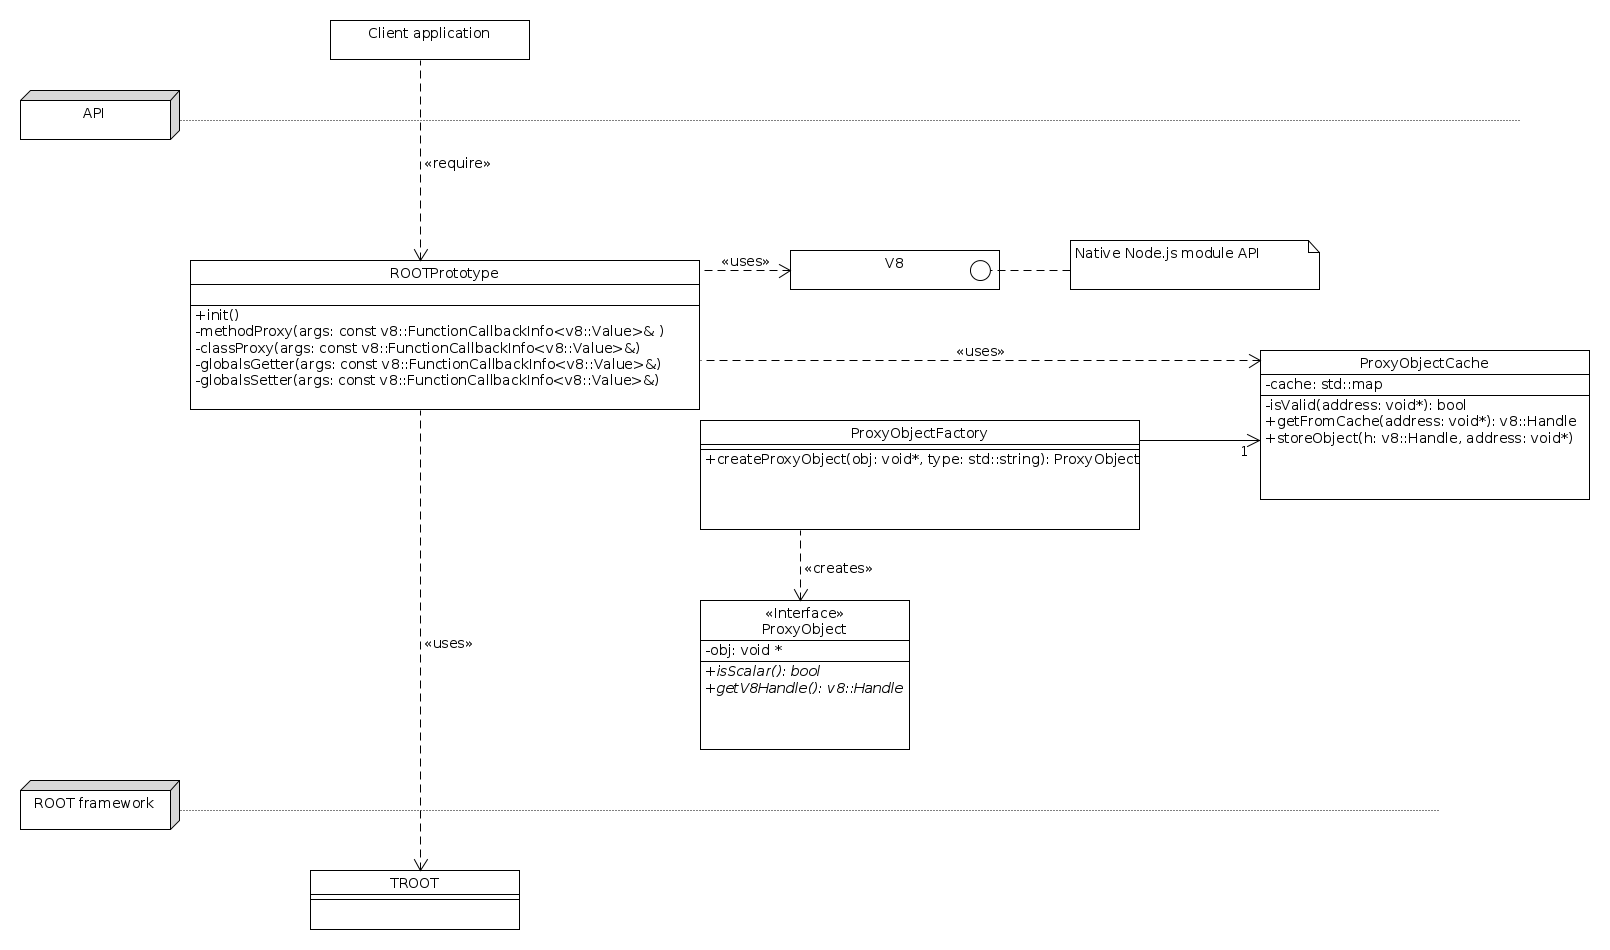
\includegraphics[width=18cm]{./latex/resources/architecture.png}
	\caption{basic architecture draft}
\end{figure}

\pagebreak[4]

\section{Dynamic Models}
The following figure shows how rootJS initializes upon being called the first time by a client application. As bindings do not add any functionality of their own, the client application is not further specified. After the bindings are initialized the client application may use any root functionality through the roootJS API.
\begin{figure}[htb]
	\centering
	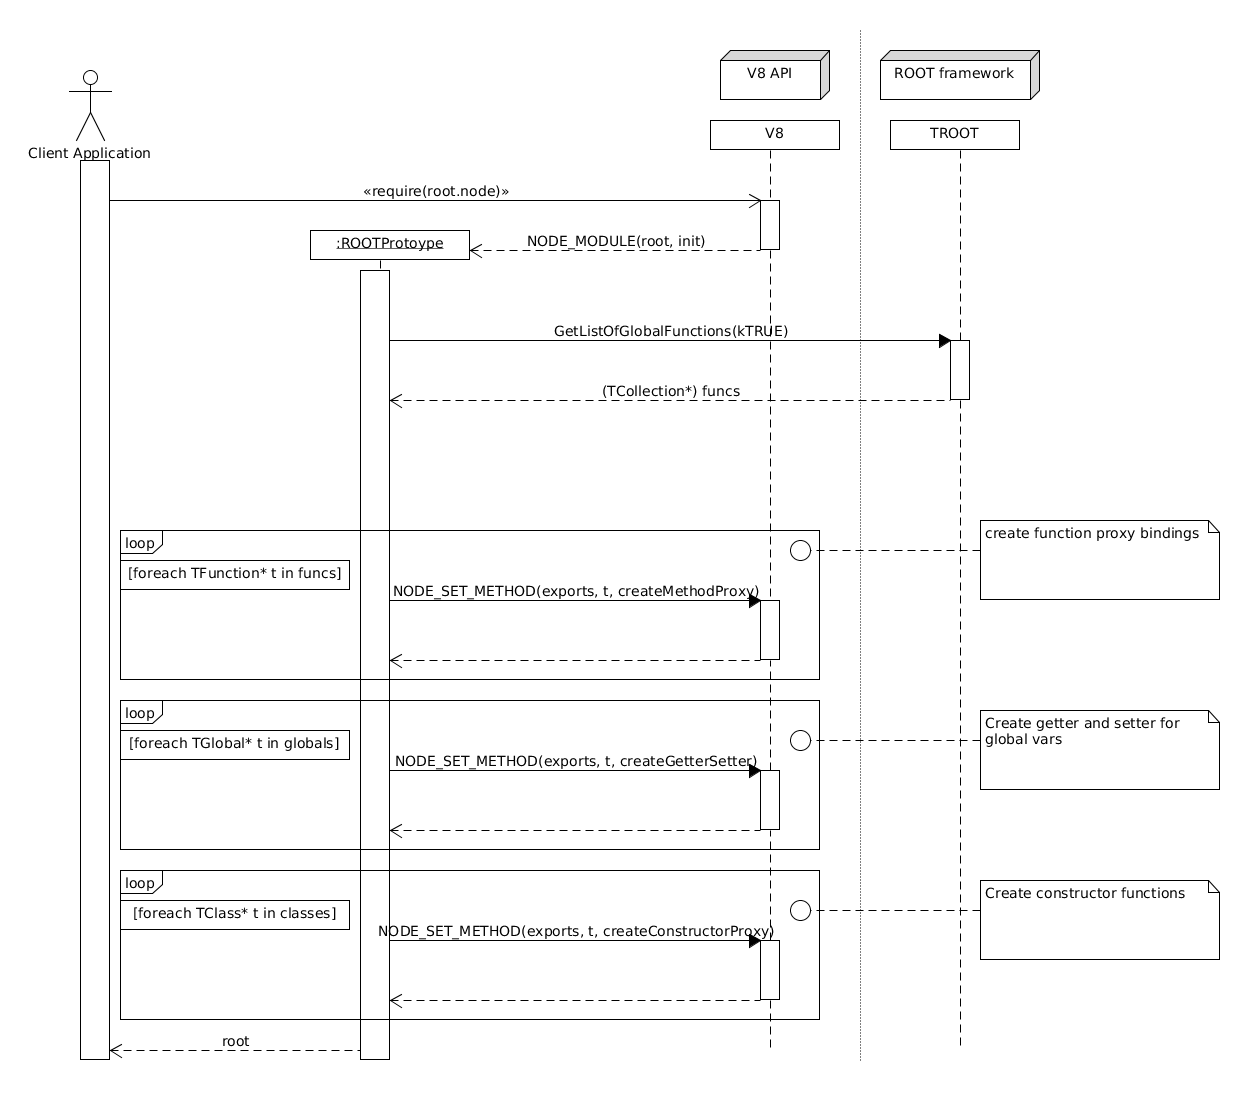
\includegraphics[width=18cm]{./latex/resources/startupSequence.png}
	\caption{startup sequence}
\end{figure}
